\documentclass[11pt]{article}
\usepackage[margin=1in]{geometry}
\usepackage{amsmath,amssymb,amsthm}
\usepackage{graphicx}
\usepackage{hyperref}

\newcommand{\DeltaG}{\Delta}
\newcommand{\eps}{\varepsilon}
\newcommand{\Gam}{\Gamma_2}
\newcommand{\clGam}{\overline{\Gamma_2}}

\newtheorem{theorem}{Theorem}
\newtheorem{lemma}{Lemma}
\newtheorem{assumption}{Conditional Dependency}
\newtheorem{corollary}{Corollary}

\title{A conditional Hilbert-factorization reduction for\\
the biased-coin Tylli problem}
\author{Automatic Math Discovery Run \texttt{fa\_banach\_001}}
\date{July 3, 2026}

\begin{document}
\maketitle

\section*{Status}

This is a conditional reduction for the final open problem in
Johnson--Schechtman \cite{JS2007}. It does not claim a full solution. It
proves that the biased-coin operator \(T_\eps\) satisfies the Tylli and Weak
Tylli conclusions once one proves a concrete uniform resolvent multiplier
estimate for one smaller biased-coin operator \(T_\delta\).

\section*{Source problem}

Johnson and Schechtman define \(T_\eps\) on \(L_p(\DeltaG)\), where
\(\DeltaG=\{-1,1\}^{\mathbb N}\) is the Cantor group with Haar measure, as
convolution by the \(\eps\)-biased coin. Equivalently, if \(w_A\) denotes the
Walsh character indexed by a finite set \(A\subset\mathbb N\), then
\[
        T_\eps w_A=\eps^{|A|}w_A .
\]
At the end of Section 5 they ask the following.

\begin{center}
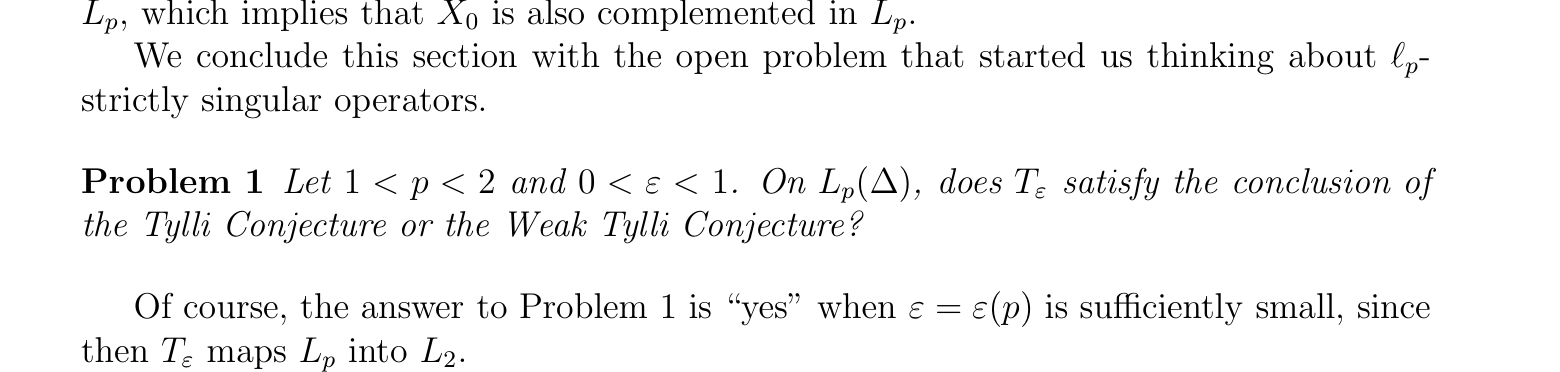
\includegraphics[width=\textwidth]{figures/open_problem_crop.png}
\end{center}

\noindent
Thus, for \(1<p<2\) and \(0<\eps<1\), the problem is whether \(T_\eps\) lies
in the norm closure of the operators factoring through Hilbert space, or at
least satisfies the corresponding Weak Tylli conclusion after composition
with an isometric embedding into \(\ell_\infty\). The source paper notes that
the answer is already yes when \(\eps\) is sufficiently small, because then
\(T_\eps:L_p(\DeltaG)\to L_2(\DeltaG)\) is bounded \cite{JS2007}.

\section*{Conditional dependency}

Fix \(1<p<2\) and \(0<\delta<1\). Let \(Q_t\) be the Walsh multiplier
\[
        Q_t w_A=\frac{t}{t+\delta^{|A|}}w_A,\qquad t>0 .
\]

\begin{assumption}[positive-resolvent Walsh multiplier bound]\label{ass:res}
There is a constant \(C=C(p,\delta)\) such that
\[
        \|Q_t\|_{L_p(\DeltaG)\to L_p(\DeltaG)}\le C
\]
for every \(t>0\).
\end{assumption}

Equivalently, \(t(tI+T_\delta)^{-1}\) is uniformly bounded on \(L_p(\DeltaG)\).
This is implied by sectoriality of \(T_\delta\) of angle \(<\pi\), but the
packet records the smaller estimate actually used in the proof.

\section*{Idea of the proof}

Choose \(\delta<\eps\) so small that \(T_\delta:L_p\to L_2\) is bounded.
Then \(T_\delta\) factors through Hilbert space. Put
\[
        \alpha=\frac{\log\eps}{\log\delta}\in(0,1),
\]
so that \(\delta^\alpha=\eps\). The multiplier bound lets us form the
Balakrishnan root integral
\[
        B_\alpha=
        \frac{\sin(\pi\alpha)}{\pi}\int_0^\infty
        t^{\alpha-1}T_\delta(tI+T_\delta)^{-1}\,dt
\]
in operator norm. Each integrand still factors through Hilbert space, because
it is \(T_\delta\) followed by a bounded operator. On each Walsh character the
scalar integral gives \((\delta^{|A|})^\alpha=\eps^{|A|}\), so \(B_\alpha\)
is exactly \(T_\eps\). Thus the only missing ingredient is the uniform
resolvent multiplier estimate.

\begin{lemma}[Balakrishnan multiplier under Assumption \ref{ass:res}]
\label{lem:bal}
Assume \ref{ass:res}. For every \(0<\alpha<1\), the operator
\[
        B_\alpha=
        \frac{\sin(\pi\alpha)}{\pi}\int_0^\infty
        t^{\alpha-1}T_\delta(tI+T_\delta)^{-1}\,dt
\]
is a well-defined bounded operator on \(L_p(\DeltaG)\), with convergence in
operator norm, and
\[
        B_\alpha w_A=(\delta^{|A|})^\alpha w_A
\]
for every Walsh character \(w_A\).
\end{lemma}

\begin{proof}
Assumption \ref{ass:res} gives boundedness of \(Q_t=t(tI+T_\delta)^{-1}\).
Hence
\[
        T_\delta(tI+T_\delta)^{-1}=I-Q_t
\]
is bounded uniformly for \(0<t\le1\). This gives integrability near \(0\),
because \(t^{\alpha-1}\) is integrable there. For \(t\ge1\),
\[
        T_\delta(tI+T_\delta)^{-1}=t^{-1}T_\delta Q_t,
\]
so its norm is at most \(t^{-1}\|T_\delta\|\,C\), and
\(t^{\alpha-2}\) is integrable at infinity. Therefore the Bochner integral
converges in operator norm.

On the one-dimensional span of a Walsh character \(w_A\), the integral reduces
to the classical scalar identity
\[
        \frac{\sin(\pi\alpha)}{\pi}
        \int_0^\infty t^{\alpha-1}\frac{\lambda}{t+\lambda}\,dt
        =\lambda^\alpha,\qquad \lambda>0,\quad 0<\alpha<1,
\]
with \(\lambda=\delta^{|A|}\). This proves the asserted action on Walsh
characters.
\end{proof}

\begin{theorem}[conditional Hilbert-factorization conclusion]
\label{thm:conditional}
Let \(1<p<2\) and \(0<\delta<\eps<1\). Assume that
\(T_\delta:L_p(\DeltaG)\to L_2(\DeltaG)\) is bounded and that Assumption
\ref{ass:res} holds for this \(\delta\). Then
\[
        T_\eps\in \clGam(L_p(\DeltaG)),
\]
the norm closure of the operators on \(L_p(\DeltaG)\) that factor through
Hilbert space. Consequently \(T_\eps\) satisfies the Tylli conclusion and the
Weak Tylli conclusion.
\end{theorem}

\begin{proof}
Since \(T_\delta:L_p\to L_2\) is bounded and the inclusion
\(L_2(\DeltaG)\hookrightarrow L_p(\DeltaG)\) is bounded on a probability
space when \(p<2\), \(T_\delta\) factors through the Hilbert space
\(L_2(\DeltaG)\). Let \(S=T_\delta\).

Set \(\alpha=\log\eps/\log\delta\). Because \(0<\delta<\eps<1\), we have
\(0<\alpha<1\), and \(\delta^\alpha=\eps\). By Lemma \ref{lem:bal},
\[
        B_\alpha=
        \frac{\sin(\pi\alpha)}{\pi}\int_0^\infty
        t^{\alpha-1}S(tI+S)^{-1}\,dt
\]
is bounded on \(L_p(\DeltaG)\) and satisfies
\[
        B_\alpha w_A=(\delta^{|A|})^\alpha w_A=\eps^{|A|}w_A
        =T_\eps w_A.
\]
Walsh polynomials are dense in \(L_p(\DeltaG)\), and both \(B_\alpha\) and
\(T_\eps\) are bounded, so \(B_\alpha=T_\eps\).

It remains to check that \(B_\alpha\) belongs to the closed Hilbert-factor
ideal. For each \(t>0\), the operator
\[
        S(tI+S)^{-1}=S Q_t/t
\]
factors through Hilbert space because \(S\) does and \(Q_t/t\) is a bounded
operator on \(L_p\). The integral defining \(B_\alpha\) is the norm limit of
Riemann sums of such Hilbert-factor operators. Since \(\clGam(L_p)\) is a
closed operator ideal, \(B_\alpha\in\clGam(L_p)\).

This proves the Tylli conclusion. If \(J:L_p(\DeltaG)\to\ell_\infty\) is an
isometric embedding, then \(JT_\eps\) is the norm limit of the compositions of
\(J\) with Hilbert-factor operators. Thus \(JT_\eps\) lies in the closure of
the operators from \(L_p(\DeltaG)\) to \(\ell_\infty\) that factor through
Hilbert space, which is the Weak Tylli conclusion.
\end{proof}

\begin{corollary}[what remains for a full solution]
For fixed \(1<p<2\), if Assumption \ref{ass:res} holds for some
\(\delta>0\) for which \(T_\delta:L_p(\DeltaG)\to L_2(\DeltaG)\) is bounded,
then every \(T_\eps\), \(\delta<\eps<1\), has an affirmative answer to the
Johnson--Schechtman problem.
\end{corollary}

\section*{Verification and novelty notes}

The proof is purely analytic after Assumption \ref{ass:res}. The verification
focus is therefore the multiplier family \(m_t(n)=t/(t+\delta^n)\). A bounded
sectorial functional calculus for \(T_\delta\) would imply the assumption, but
standard Ritt/Stolz calculi for sampled semigroups do not by themselves give
the needed root \(z^\alpha\), because \(z^\alpha\) is not holomorphic at
\(0\) when \(0<\alpha<1\).

Cheap run-index searches found no previous packet for arXiv:0708.0560. The
nearby Johnson--Schechtman closed-ideal packets concern other strictly
singular operators and do not answer this biased-coin problem. A bounded
local and web search for the exact biased-coin/Tylli phrases found the source
problem and relevant functional-calculus background, but no later explicit
answer to this question.

\section*{References}

\begin{thebibliography}{9}

\bibitem{JS2007}
W. B. Johnson and G. Schechtman,
\emph{Multiplication operators on \(L(L_p)\) and \(\ell_p\)-strictly singular
operators}, arXiv:0708.0560.

\bibitem{LeMerdy2012}
C. Le Merdy,
\emph{\(H^\infty\) functional calculus and square function estimates for
Ritt operators}, arXiv:1202.0768.

\bibitem{Schwenninger2015}
F. L. Schwenninger,
\emph{Functional calculus estimates for Tadmor--Ritt operators},
arXiv:1507.00049.

\end{thebibliography}

\end{document}
